\documentclass{VUMIFPSkursinis}
\usepackage{algorithmicx}
\usepackage{algorithm}
\usepackage{algpseudocode}
\usepackage{amsfonts}
\usepackage{float}
\usepackage{amsmath}
\usepackage{bm}
\usepackage{caption}
\usepackage{color}
\usepackage{float}
\usepackage{graphicx}
\usepackage{listings}
\usepackage{subfig}
\usepackage{ltablex}
\usepackage{longtable}
\usepackage{wrapfig}
\usepackage{enumitem}
\usepackage{subfig}
\usepackage{pbox}
\renewcommand{\labelenumii}{\theenumii}
\renewcommand{\theenumii}{\theenumi.\arabic{enumii}.}
\renewcommand{\labelenumiii}{\theenumiii}
\renewcommand{\theenumiii}{\theenumii\arabic{enumiii}.}
% Titulinio aprašas
\university{Vilniaus universitetas}
\faculty{Matematikos ir informatikos fakultetas}
\department{Programų sistemų katedra}
\papertype{Projektinis darbas}
\title{Internetinio banko tinklalapis}
\titleineng{Bankininkystė}
\status{3 kurso 3 grupės studentai}
\author{Justas Tvarijonas}
\secondauthor{Džiugas Mažulis}   
\thirdauthor{Michal Stankevič}   
\supervisor{Kristina Lapin, Doc., Dr.}
\date{Vilnius – \the\year}

\begin{document}
\maketitle
\sectionnonum{Anotacija}
\subsectionnonum{Darbo tikslas}
Naudojant į vartotoją orientuotą dizainą palengvinti bei pagerinti Swedbank internetinio banko puslapio naudojamumą bei efektyvumą taip padidinant puslapio našumą bei vartotojų pasitenkinimą.
\subsectionnonum{Darbo pasiskirstymas}
\begin{itemize}
	\item Justas Tvarijonas - tvarijonasjustas@gmail.com \newline
	Įvadas, kompiuterizuojamų veiklų analizė, įkvepiantys interfeisai.
	\item Džiugas Mažulis - džiugas.mažulis@gmail.com \newline 
	Kompiuterizuojamų veiklų analizė, įkvepiantys interfeisai.
	\item Michal Stankevič - michal.stankevic@gmail.com \newline
	 Kompiuterizuojamų veiklų analizė, įkvepiantys interfeisai.
\end{itemize}
\tableofcontents
\sectionnonum{Įvadas}
\subsectionnonum{Dalykinė sritis}
Internetinė bankininkystė.
\subsectionnonum{Probleminė sritis}
Vartotojo grafinės sąsajos išmokstamumo gerinimas, pagrindinėms funkcijoms pasiekti atliekamų žingsnių bet klaidų mažinimas.
\subsectionnonum{Naudotojai}
Banko klientas - turi galimybę atlikti mokėjimus, peržiūrėti sąskaitos išrašus, kurti mokėjimo ruošinius, ieškoti reikalingos informacijos.
\subsectionnonum{Darbo pagrindas}
Pirmojo laboratorinio darbo reikalavimai.
\section{Būsimos sistemos įtakojamų asmenų kategorijos}
\subsection{Suinteresuotų asmenų grupės}
\begin{itemize}
	\item Pirminiai - Banko klientai, betarpiškai naudojasi sistema.
	\item Antriniai - neegzistuoja.
	\item Tretiniai - SEB, Luminor - bankai kurių klientų skaičių įtakoja šio banko kokybinės charakteristikos, bei naujai pritraukiamų klientų skaičius. Akcininkai, kurių pajamos priklauso nuo banko klientų skaičiaus.
\end{itemize}
\section{Banko klientų poreikiai}
\subsection{Naudotojų charakteristikos}
\subsubsection{Informacinių technologijų priemonės}
\begin{itemize}
	\item Išmanusis telefonas (naršyklė bei Smart-ID).
	\item Asmeninių kompiuterių naršyklės.
	\item Planšetinių kompiuterių naršyklės.
\end{itemize}
\subsubsection{Motyvacija ir galimybės tobulinti įgūdžius}
\begin{itemize}
	\item Motyvacija - didelė (pasirašyta sutartis su banku).
	\item Klientai turi skirtingus IT įgūdžius.
	\item Klientai skirtingais dažnumais naudojasi elektronine bankininkyste.
\end{itemize}
\subsubsection{Veiklų kontekstai}
\begin{itemize}
	\item Veikla yra pertraukiama. Klientas gali suformuluoti mokėjimą, tada užsiimti kita veikla ir vėliau grįžti užbaigti mokėjimą.
	\item Mokėjimai atliekami su dideliu susikaupimu.
	\item Naudojimasis sistema atliekamas saugioje aplinkoje.
	\item Paprastai sistema naudojama turint aiškų tikslą.
	\item Apsilankymas banko svetainėje paprastai trunka iki 30 minučių.
	\item Banko klientai svetainėje apsilanko bent kelis kartus į mėnesį.
\end{itemize}
\subsubsection{Naudotojų tipas}
\begin{itemize}
	\item Naujokai - šie naudotojai iš anksto nežino kur jiems reikia spausti norint pasiekti norimą tikslą. Juos gąsdina sudėtingas ir pilnas funkcionalumo pagrindinis langas, tačiau pastebi didesnius mygtukus ar užrašus, kurie skelbia jiem naudingą informaciją.
	\item Vidutiniškai patyrę - šie naudotojai banko paslaugomis naudojasi pakankamai dažnai, kad efektyviai atliktų įprastus veiksmus, tačiau susiduria su problemomis norėdami atlikti sudėtingesnes operacijas.
	\item Ekspertai - šie sistemos naudotojai puikiai išmano sistemą, jiems patogus didelio funkcionalumo sudėtingas interfeisas. Juos erzina didelis žingsnių skaičius bei į naujokus orientuota vartotojo sąsaja.
\end{itemize}
\subsection{Kompiuterizuojamų veiklų analizė}
\subsubsection{Mokėjimo pavedimų koncepcinis scenarijus}
Kęstas nori pervesti pinigus į draugo sąskaitą, tačiau pagrindiniame lange neranda pinigų pavedimo funkcijos. Nežinodamas ar „Vietiniai mokėjimai“ yra tai, ko jam reikia, jis meniu juostoje paspaudžia „Mano bankas“. Neradęs tinkamo pasirinkimo Petras meniu juostoje spusteli „Kasdieninės paslaugos“, tačiau jį suglumina skiltyje „Mokėjimai“ atsiradę pasirinkimai: „Mokėjimo pavedimai“, „Vietiniai mokėjimai“, „Įmokos“, „E. sąskaitos“. Pasirinktame „Mokėjimo pavedimai“ lange klientas nežino ką įvesti „Gavėjo pavadinimas“ skiltyje, tik paspaudęs ant klaustuko simbolio sužino, jog įvesti reikia draugo vardą ir pavardę. Visą sąskaitos numerį Petras turi vesti ranka, nors jau yra ankščiau pervedęs draugui pinigų. Įvedęs visus duomenis bei paspaudęs toliau vartotojas atsiduria vietinių mokėjimų lange, kuriame turi įvesti gavėjo šalį, adresą. Paspaudęs mygtuką „Toliau“ Petras perveda draugui pinigus.
\subsubsection{Mokėjimo pavedimų veiklų charakteristikos}
Veiklos dažnis: mokėjimo pavedimai yra esminė bei dažniausiai naudojama elektroninės bankininkystės funkcija: apie 10-15 kartų per mėnesį. Privaloma užtikrinti akivaizdų, vienprasmišką bei vieno mygtuko paspaudimu pasiekiamą pagrindinį funkcionalumą norint greitai ir rezultatyviai atlikti pavedimus. Įvesties langai turi būti aiškiai suprantami bei pasirinkus siųsti pinigus sistema privalo pasiūlyti pasirinkti gavėją iš gavėjų sąrašo arba ankstesnių gavėjų. Iš banko sąskaitos galima atpažinti gavėjo šalį, todėl sistema neturėtų reikalauti šio parametro. \par 
Veiklos trukmė: mokėjimo pavedimas internetinės bankininkystės sistemoje užtrunka nuo 2 iki 5 minučių.
\subsubsection{Mokėjimo pavedimų problemos ir tobulinimo galimybės}
\begin{itemize}
	\item Mokėjimo pavedimo funkcija vizualiai neatkreipia dėmesio bei yra neaiškaus pavadinimo.
	\item Mokėjimų skiltyje per daug pavedimo interpretacijų.
	\item Įvesties lauko „Gavėjo pavadinimas“ pavadinimas neaiškiai apibrėžia reikalaujamus duomenis.
	\item Sistema neteikia galimybės pasirinkti anksčiau naudotą gavėją arba gavėją iš sąrašo.
	\item Sistema iš banko sąskaitos neatpažįsta gavėjo šalies.
\end{itemize}
\subsubsection{Būsimasis patobulintas scenarijus}
\begin{center}
\textbf{Vartotojas norėdamas atlikti mokėjimo pavedimą:}
\end{center}
\begin{enumerate}
	\item Vartotojas įveda pinigų sumą
	\item Sistema pateikia gavėjų sąrašą, kuriame nurodomi gavėjų vardai ir banko sąskaitos, galimybę įvesti gavėjo duomenis 
	\item Vartotojas įvesdamas duomenis
\begin{enumerate}
	\item Pasirenka gavėją iš gavėjų sąrašo
	\item Pasirenka įvesti duomenis
\begin{enumerate}
	\item Sistema pavaizduoja mokėjimo formą
	\item Vartotojas įveda gavėjo duomenis
\end{enumerate}
\end{enumerate}
	\item Vartotojas patvirtina mokėjimą
	\item Sistema rodo mokėjimo patvirtinimą
\end{enumerate}
\subsubsection{Informacijos paieškos koncepcinis scenarijus}
Jonas ieško kaip gali išsinuomuoti saugyklą banke, pasirinkęs "Mano bankas" pamato ilgą sarašą informacijos, tačiau jį peržvelgęs nerando norimos informacijos, dar kartą atydžiai peržvelgia naudingos informacijos nuorodų grupę, tačiau vistiek neranda norimo puslapio nuorodos. Tik tada pamato, kad dešiniąjame lango kampe yra paieškos logotipas, jį paspaudus įveda "seifo nuoma" į paieškos langą, tačiau paieška neranda nieko prasmingo. Galiausiai neapsikentęs jis parašo žinutę banko dorbuotojui, kuris jam atsiunčia nuorodą į ieškomą puslapį, bei praneša, kad šios informacijos reikia ieškoti neprisijungus prie banko. 
\subsubsection{Informacijos paieškos veiklų charakteristikos}
Veiklos dažnis: Informacijos paieška banko internetinėje svetainėje paprastai nėra dažna: apie 5-6 kartus į metus, todėl jos pasiekimas turėtų būti pakankamai akivaizdus. Neradus rezultatų siūlytų panašius arba atidaryti bendravimo gyvai langą, kuriame vartotojas galėtų sužinoti norimą informaciją. \par
Veiklos trukmė: Informacijos paieška vidutiniškai užtrunka neilgai - iki 5 minučių.
\subsubsection{Informacijos paieškos problemos ir tobulinimo galimybės}
\begin{itemize}
	\item Paieškos lango pozicija nėra akivaizdi.
	\item Paieškos rezultatų negalima sugrupuoti.
	\item Paieška informacijos ieško ne iš viso galimo informacinio lauko.
	\item Neradus rezultatų nėra pasiūlomas joks situacijos sprendimas.
	\item Atidarius vieną iš variantų, vartotojui nėra galimybė mygtuko paspaudimu sugrįžti atgal.
\end{itemize}
\subsubsection{Būsimasis patobulintas scenarijus}
\begin{center}
	\textbf{Vartotojas norėdamas surasti informacijos apie seifų nuoma:}
\end{center}
\begin{enumerate}
	\item Paspaudžia ant paieškos mygtuko pagrindiniame lange
	\item Sistema atidaro naują langą, kuriame vartotojas gali įvesti raktinius žodžius
	\item Vartotojas įvedęs raktinius žodžius gali atidaryti vieną iš rastų rezultatų, filtruoti rezultatus pagal kategorijas, pažiūrėti alternatyvius siūlomus raktinius žodžius.
	\begin{enumerate}
		\item atidarius vieną iš rezultatų:
		\begin{enumerate}
			\item tame pačiame lange atidaromas pasirinkto rezultato puslapis
			\item vartotojas vienu paspaudimu gali grįžti atgal į rezultatų sąrašą
		\end{enumerate}
	\end{enumerate}
	\begin{enumerate}
		\item pasirinkęs filtravimą pagal kategoriją: vartotojas mato tik tuos rezultatus, kurie priklauso pasirinktai kategorijai.
		\begin{enumerate}
			\item vartotojas mato tik tuos rezultatus, kurie priklauso pasirinktai kategorijai
			\item vartotojas bet gali atšaukti filtravimą
		\end{enumerate}
	\end{enumerate}
	\begin{enumerate}
		\item pasirinkęs peržiūrėti alternatyvius siūlomus variantus:
		\begin{enumerate}
			\item Sistema parodo siūlomus variantus
			\begin{enumerate}
			\item gali pasirinkti vieną iš siūlomų variantų ir ieškoti iš naujo
			\item toliau žiūrėti jau rastus rezultatus
			\end{enumerate}
		\end{enumerate}
	\end{enumerate}
\end{enumerate}
\subsubsection{Mokėjimo ruošinio sukūrimo koncepcinis scenarijus}
Antanas nori sukurti mokėjimo ruošinį pagal seniau atliktą mokėjimą, tačiau, kadangi nežino, kaip tai atlikti jis bando orientuotis pagal pavadinimus. Pasirinkęs kasdienes paslaugas ir peržvelges visus variantus per kelias minutes randa pasirinkimą "Mokėjimo ruošiniai" bei ant jo paspaudžia. Atsidariusiame lange pasirenka "Sukurti vietinį mokėjimo ruošinį", tačiau atsidarius naujam langui pamato, kad nebus pasirinkimo sukurti ruošinį pagal buvusį mokėjimą, todėl, norėdamas sužinoti gavėjo duomenis, nueina peržvelgti buvusius mokėjimus. Ten susiradęs reikiamą mokėjimą pamato, kad gali sukurti ruošinį pagal šį mokėjimą, taip ir padaro.
\subsubsection{Mokėjimo ruošinio sukūrimo veiklų charakteristikos}
Veiklos dažnis: Mokėjimo ruošinio sukūrimas yra retas veiksmas, todėl vartotojas kiekvieną kartą jį atlieka kaip iš naujo, todėl jis turėtų būti pakankamai aiškus ir paprastas. \par
Veiklos trukmė: Mokėjimo ruošinio sukūrimas turėtų užtrukti iki 10 minučių.
\subsubsection{Mokėjimo ruošinio sukūrimo problemos ir tobulinimo galimybės}
\begin{itemize}
	\item Mokėjimo ruošinių lange nėra pasirinkimo sukurti ruošinį pagal buvusius mokėjimus
	\item Mokėjimo ruošinių paieška galima tik pagal jo pavadinima (tačiau ne pagal gavėją bei mokėjimo paskirtį)
\end{itemize}
\subsubsection{Būsimasis patobulintas scenarijus}
\begin{center}
	\textbf{Vartotojas norėdamas sukurti mokėjimo ruošinį:}
\end{center}
\begin{enumerate}
	\item atsidaro mokėjimo ruošinių langą bei pasirenka sukurti vietinį mokėjimo ruošinį.
	\item Sistema vartotojui duoda pasirinkima kurti mokėjimo ruošinį pagal buvusį mokėjimą arba kurti be jo.
	\begin{enumerate}
		\item Vartotojui pasirinkus kurti ruošinį pagal buvusį mokėjimą:
		\begin{enumerate}
			\item Sistema vartotojui atidaro naują langą, kuria rodomi buvę Mokėjimai
			\item Vartotojas susirandą norimą mokėjimą bei jį pasirenka
			\item Sistema vartotoja nukelia į mokėjimo ruošinio sukurimo langą, kuriame automatiškai užpildo laukus pagal pasirinktą buvusį mokėjimą
			\item Vartotojas, patikrinęs mokėjimo ruošinio laukus, pasirenka jį išsaugoti
		\end{enumerate}
		\item Vartotojui pasirinkus kurti mokėjimo ruošinį nuo nulio:
		\begin{enumerate}
			\item Sistema vartotojui atidaro mokėjimo ruošinio sukūrimo langą, kuriame visi laukai yra tušti
			\item Vartotojas suveda reikiamus duomenis bei išsaugo mokėjimo ruošinį
		\end{enumerate}
	\end{enumerate}
\end{enumerate}
\subsubsection{Sąskaitos išrašų tikrinimo konceptualus scenarijus}
Džiugas nori pažiūrėti kelių paskutinių mėnesių sąskaitos išrašą. Prisijungęs prie internetinio banko, atitinkamuose meniu skiltyse pasirenka „Kasdienės paslaugos”, vėliau - „Išrašas”. Išrašo sukūrimui sistema reikalauja sąskaitos pavadinimo bei laikotarpio, kurio metu sąskaitoje vyko finansinės operacijos. Išrašo laikotarpį apibrėžiantys formos laukai turi numatytasiąs reikšmes: einamojo mėnesio pirmoji diena ir šiandieninė data. Tikėdamasis gauti išrašą apie kelis mėnesius sąskaitos naudojimo, Džiugas keičia pradinės datos reikšmę - spaudžia ant lauko, išskleidžiamas kalendorius, kuriame jis renkasi norimą mėnesį ir pirmą dieną. Paspaudęs „Pateikti užklausą", jis išvysta sugeneruotą išrašą. Peržvelgęs jį, Džiugas nori praplėsti laikotarpį dviem mėnesiams atgaline data. Dėl to jis privalo vėl keisti pradinės datos reikšmę: mėnesį ir dieną, nors jam užtektų pakeisti tik mėnesį.
\subsubsection{Sąskaitos išrašų tikrinimo veiklų charakteristikos}
Veiklos dažnis: Sąskaitos išrašo tikrinimo dažnis varijuoja. Įprasti klientai retai tikrina sąskaitų išrašus. 

Funkcijos pasiekiamumas: vartotojas funkciją pasiekia dviem žingsniais. Norint pakartoti veiksmą, tereikia pakeisti datą.
\subsubsection{Sąskaitos išrašų tikrinimo problemos ir tobulinimo galimybės}
Pasirinkus laikotarpio pradžios mėnesį nėra numatytosios dienos reikšmės (1). Dėl to kiekvieną kartą norint pakeistį mėnesį, reikės pasirinkti dieną. (Vidutiniškai) patyrusį vartotoją papildomo žingsnio atkartojimas erzins. Taigi tobulintinas aspektas yra numatytosios dienos pridėjimas į išrašo laikotarpio pradžią, kai pasirenkamas mėnuo.
\subsubsection{Būsimasis patobulintas scenarijus}
\begin{center}
	\textbf{Vartotojas norėdamas peržiūrėti sąskaitos išrašą:}
\end{center}
\begin{enumerate}
	\item Vartotojas prisijungia prie interneto banko
	\item Vartotojas meniu pasirenka „Išrašas"
	\item Vartotojas pasirenka norimą mėnesį, o sistema dienos reikšmę nustato „1"
	\item Vartotojas pasirenka „Pateikti užklausą"
\end{enumerate}
\subsection{Panaudojamumo siekiai ir matai}
	\textbf{Bendri:}
\begin{enumerate}
	\item Vartotojui įvedus ne mažiau, kaip 3 simbolius į paieškos langą bus siūlomi pilni paieškos tekstai
	\item Kurdamas mokėjimo ruošinį vartotojas gaus bent 2 pasirinkimus jam sukurti.
	\item Vartotojas galės įvesti sumą bei pradėti pavedimą pagrindiniame lange.
	\item Vartotojas galės pasirinkti gavėją iš gavėjų arba ankstesnių gavėjų sąrašų.
	\item Mokėjimo išrašo datos apsibrėžime nebus būtina pasirinkti dieną (užteks mėnesio).
	\item Išrašo rezultatus bus galima filtruoti bent 4 būdais.
\end{enumerate}
	\textbf{Naujokų:}
\begin{enumerate}[resume]
	\item vartotojas paieškos langą surasti gebės ne per ilgesnį laiką, nei 30 sekundžių.
	\item Vartotojas gebės atlikti pavedimą per ne ilgiau kaip 2 minutes.
	\item 97\% vartotojų gebės pirmu bandymu rasti mokėjimo pavedimo funkciją.
\end{enumerate}
	\textbf{Vidutiniškai patyrusių:}
\begin{enumerate}[resume]
	\item Naudotojas gebės filtruoti paieškos rezultatus pagal skirtingas rastas grupes
	\item Vartotojas mokėjimų išrašo langą gebės pasiekti ne per daugiau, nei 2 mygtuko paspaudymus.
	\item Mokėjimo ruošinio sukurimo langą vartotojas gebės pasiekti ne per daugiau, negu 3 mygtukų paspaudimus.
	\item 80\% vartotojų gebės rasti ieškomos informacijos.
\end{enumerate}
\textbf{Patyrusių:}
\begin{enumerate}[resume]
	\item Vartotojas gebės mokėjimo ruošinių ieškoti pagal pavadinimą, gavėją bei mokėjimo paskirtį
	\item Vartotojas, rinkdamasis gavėją iš pateiktų sąrašų, gebės atlikti pavedimą 3 mygtukų paspaudimu.
\end{enumerate}
\pagebreak
\section{Įkvepiančios esamų interfeisų idėjos}
\begin{figure}[!htb]
	\begin{center}
	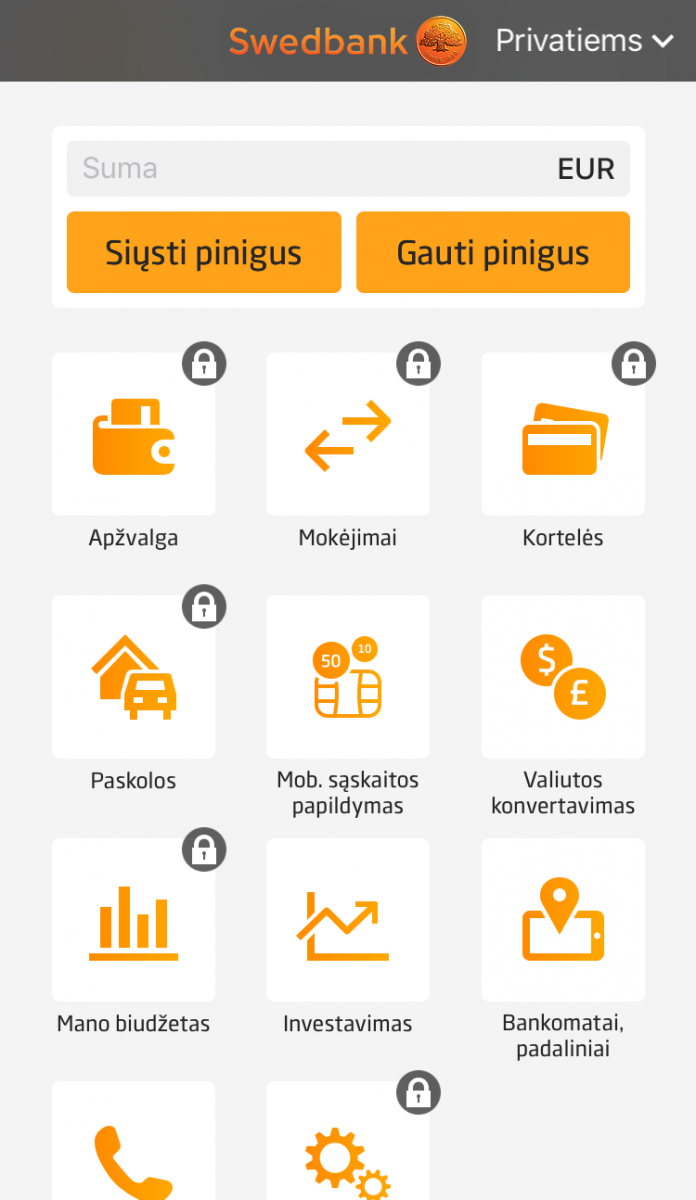
\includegraphics[scale=0.4]{mobileApp.png}
	\end{center}
  \caption{Mygtukai iš mobiliosios aplikacijos (Swedbank mobilioji programėlė)}
	\label{fig:mobileApp}
	Nauda: Suprantamesnių bei lengviau skaitomų piktogramų pagalba norimus puslapius galima rasti greičiau.
\end{figure}
\begin{figure}[!htb]
	\begin{center}
	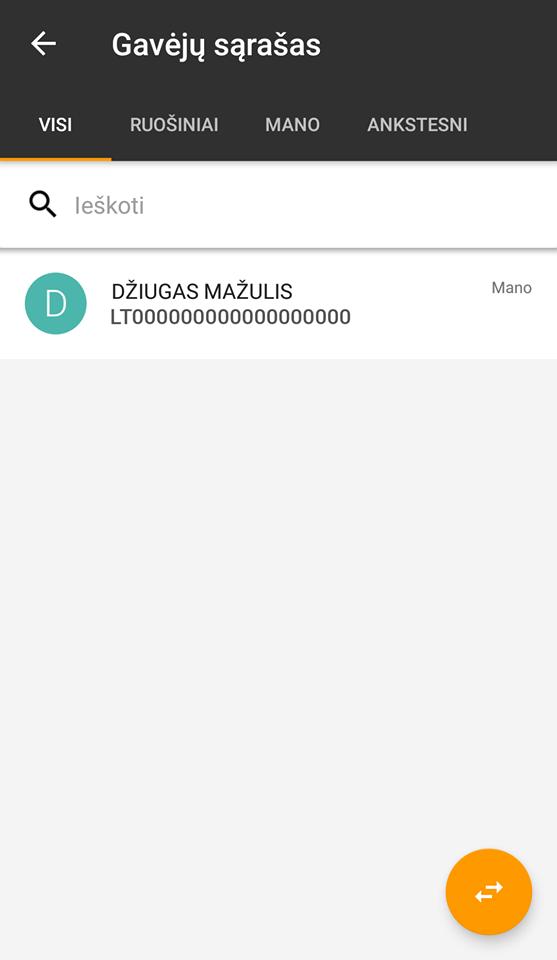
\includegraphics[scale=0.4]{mobileAppRecipientList.png}
	\end{center}
  \caption{Gavėjų sąrašas aplikacijoje (Swedbank mobilioji programėlė)}
	\label{fig:mobileAppRecipientList}
	Nauda: Galima pasirinkti gavėją iš sąrašo.
\end{figure}
\begin{figure}[!htb]
	\begin{center}
	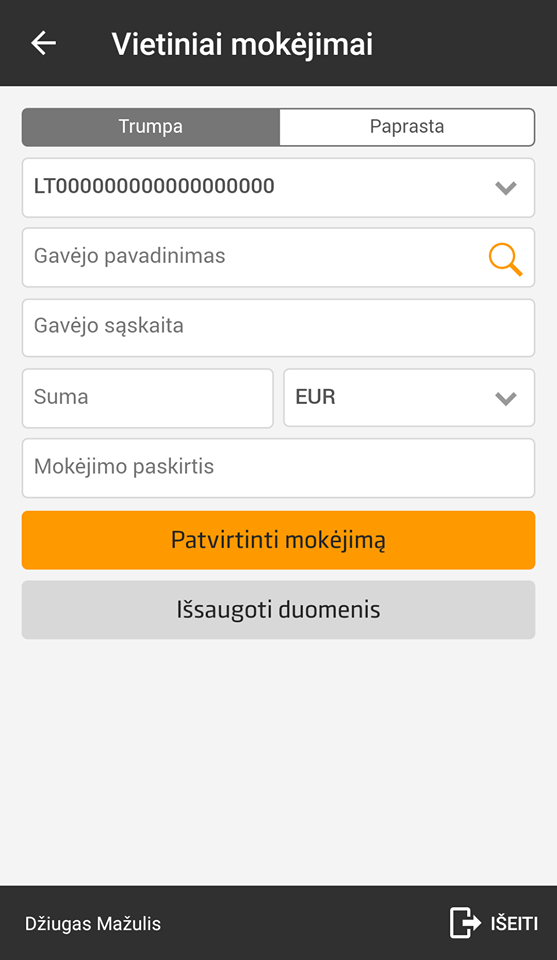
\includegraphics[scale=0.4]{mobileAppPaymentForm.png}
	\end{center}
  \caption{Mokėjimo forma aplikacijoje (Swedbank mobilioji programėlė)}
	\label{fig:mobileAppPaymentForm}
	Nauda: Būtina įvesti tik esminę informaciją.
\end{figure}
\begin{figure}[!htb]
  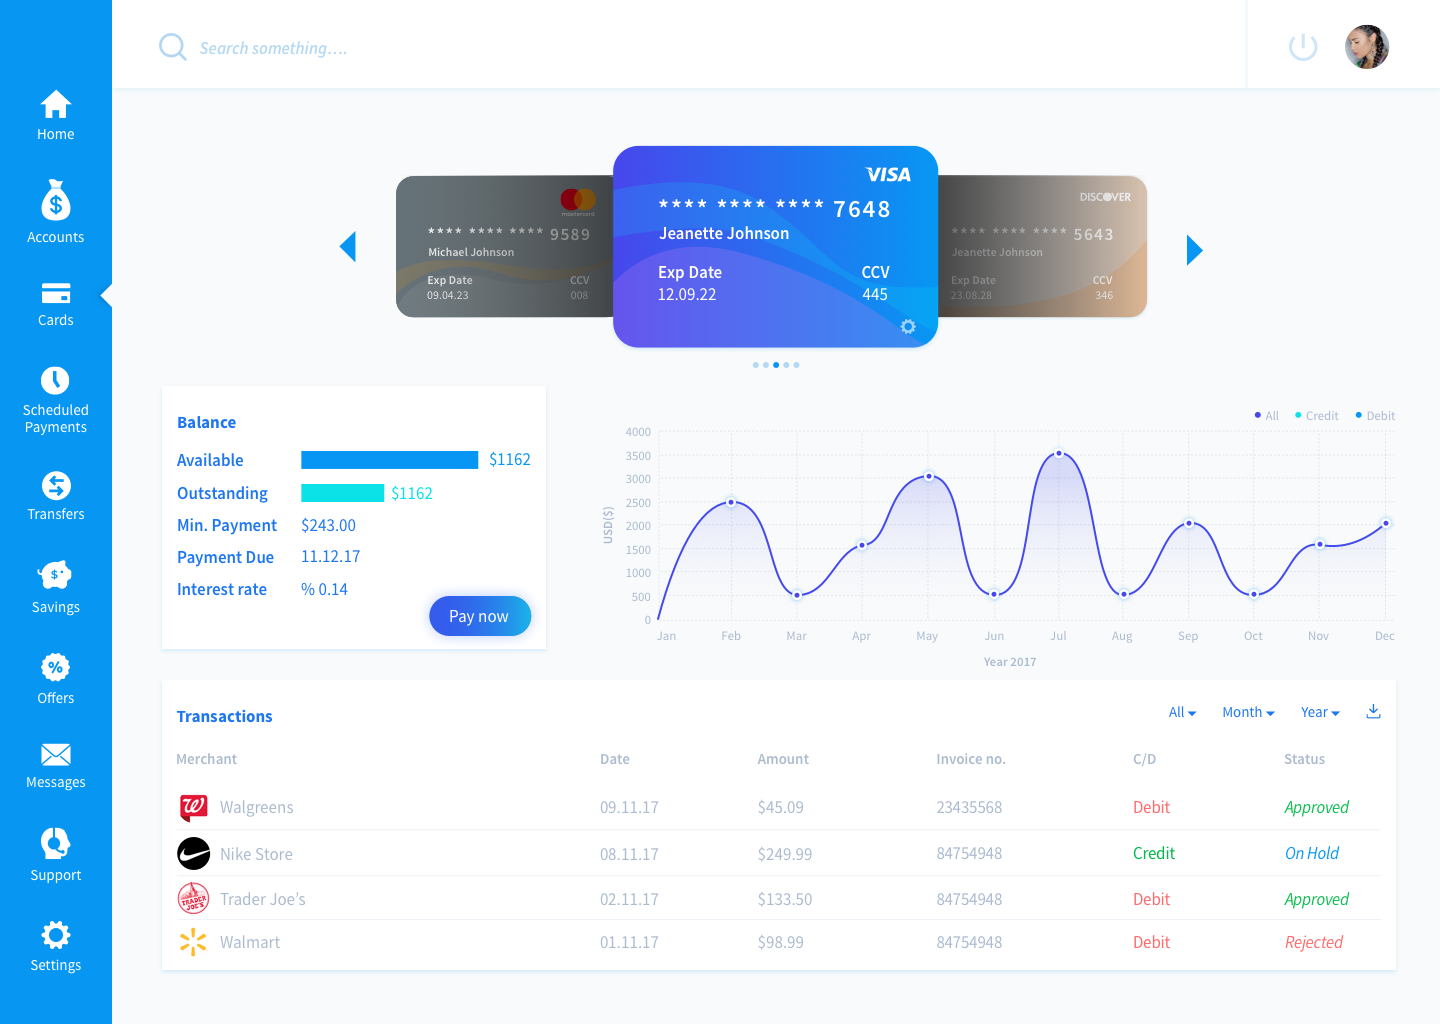
\includegraphics[width=\linewidth]{iconPlacement.png}
  \caption{Mygtukų išdėstymas svetainėje (www.unibank.com)}
	\label{fig:iconPlacement}
	Nauda: Vartotojui aiškus meniu, greitas vaikščiojimas tarp puslapių.
\end{figure}
\begin{figure}[!htb]
  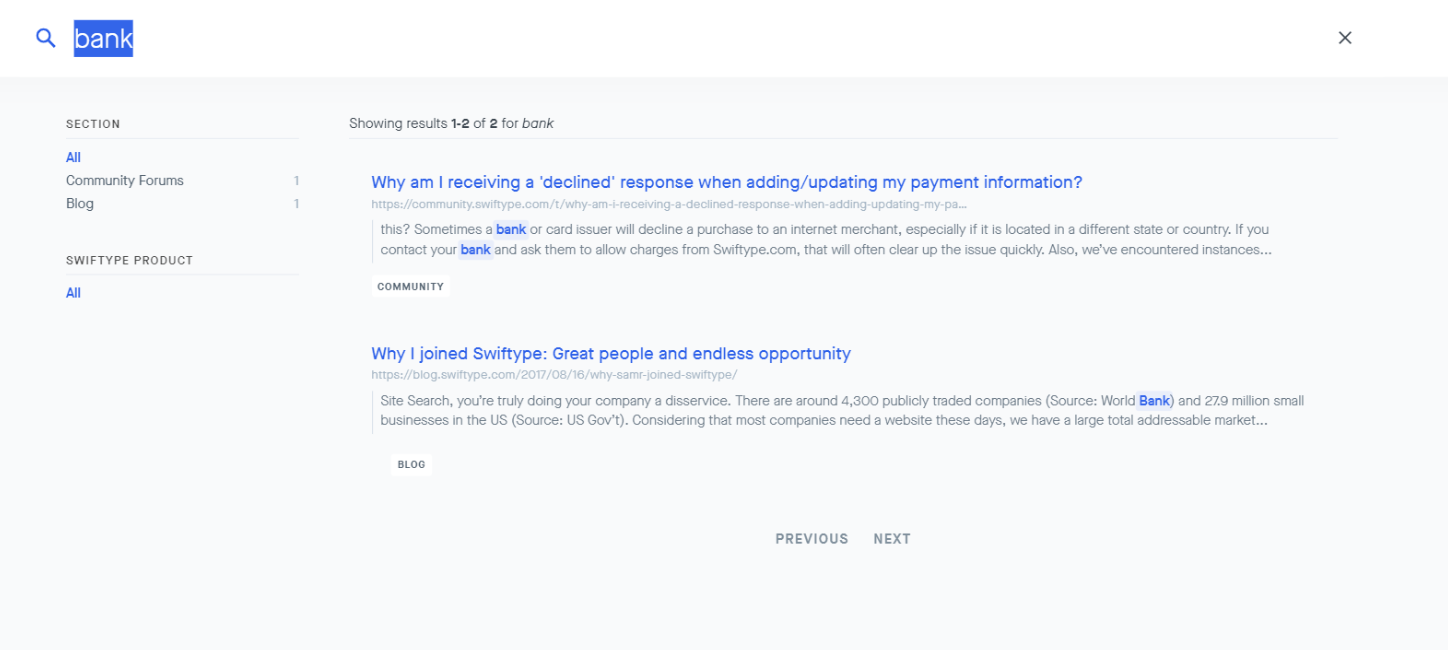
\includegraphics[width=\linewidth]{SearchWindow.png}
  \caption{Informacijos paieškos langas (swiftype.com)}
	\label{fig:searchWindow}
	Nauda: Vendant tekstą ieškoma po kiekvieno įvesto simbolio, galima filtruoti pagal skirtingas grupes.
\end{figure}
\begin{figure}[!htb]
	\begin{center}
	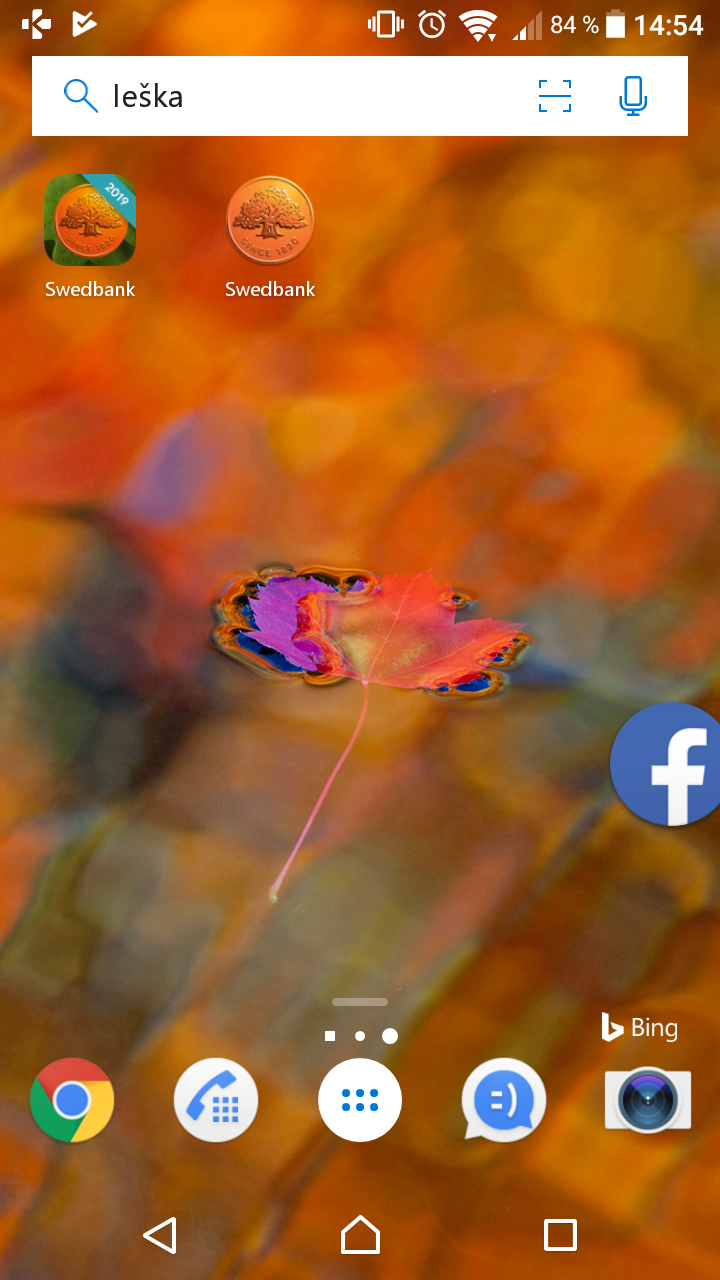
\includegraphics[scale=0.2]{pagalbaGyvai.png}
	\end{center}
  \caption{Piktograma susisiekimui su pagalba gyvai (Messenger programėlė)}
	\label{fig:pagalbaGyvai}
	Nauda: greitas pagalbos naudojantis puslapiu pasiekimas, piktogramą galima nesunkiai patraukti.
\end{figure}
\begin{figure}[!htb]
	\begin{center}
		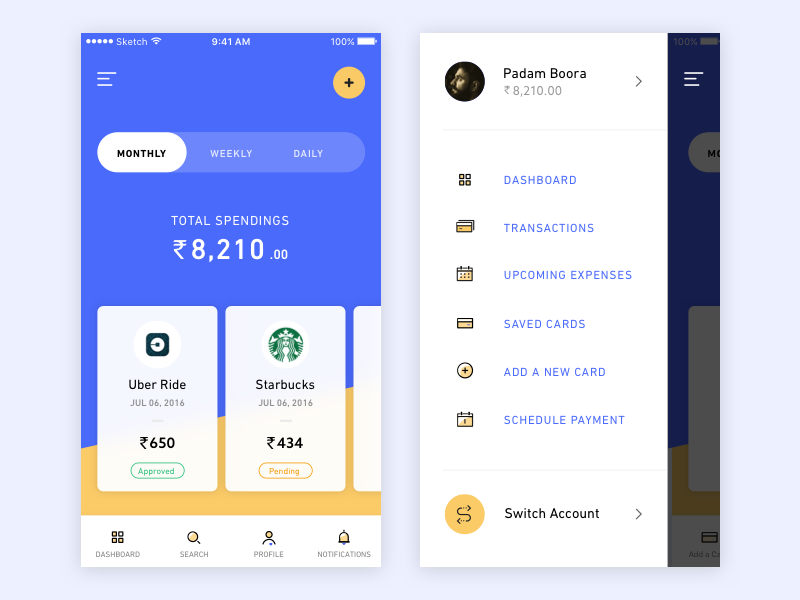
\includegraphics[scale=0.5]
		{account_report.png}
	\end{center}
	\caption{Sąskaitos apžvalga}
	\label{fig:saskaitosApzvalga}
	Nauda: patraukli ir efektyvi sąskaitos išrašo peržiūra.
\end{figure}
\begin{figure}[!htb]
	\begin{center}
		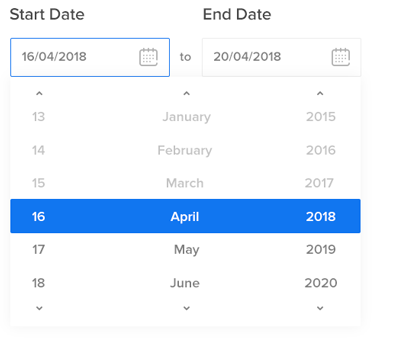
\includegraphics
		{calendar.png}
	\end{center}
	\caption{Datos pasirinkimas (sj.se)}
	\label{fig:calendar}
	Nauda: Aiškus, greitas pasirinkimas, nereikia papildomų paspaudimų keičiant tik mėnesį/metus.
\end{figure}
\end{document}
